Ao refletir sobre esse estudo, nos deparamos de volta com um panorama onde a observação fenomenológica se encontra com a tecnificação das mãos — um domínio onde a interação humana e a análise computacional convergem. Por um lado, a rede social Colab desdobra-se como um campo fértil onde as opiniões e estímulos dos usuários dispersam-se, dando vida a padrões de engajamento e ressonância. Por outro, nós, os pesquisadores, emergimos não apenas como observadores, mas como participantes ativos na interpretação dessa realidade, empregando a tecnologia para desvendar os fenômenos subjacentes às interações dos usuários. O desafio e, simultaneamente, o potencial dessa abordagem, residem na capacidade de compreender as múltiplas facetas da experiência digital e seu impacto sobre a esfera pública.

A proposta desse estudo foi sempre de ultrapassar a análise de dados; nós procuramos compreender as dinâmicas ocultas que configuram o diálogo cívico, as correntes de opinião que direcionam decisões coletivas e a dinâmica da participação política no contexto digital. O empenho em cartografar as câmaras de eco e os comportamentos polarizadores reflete uma imersão profunda na complexidade das interações sociais, evidenciando como essas estruturas virtuais refletem e, em alguns casos, intensificam as divisões presentes no nosso contexto político e social.

Os efeitos desses fenômenos são variados: no contexto cívico, percebe-se que as câmaras de eco podem tanto cristalizar o debate público quanto estimular a ação coletiva. No plano governamental, as percepções advindas desta análise fornecem ferramentas para desfazer nós de polarização e fomentar um diálogo mais abrangente e produtivo. De forma mais geral, os frutos desta pesquisa apontam para vias de fortalecimento de uma prática democrática mais sólida e aberta, que valorize e promova a diversidade de perspectivas.

Essa reflexão também nos leva a pensar sobre a relevância de examinar não só os dados que circulam pelas redes, mas também as ferramentas que nos capacitam a realizar tal exame. A instrumentalização tecnológica que guiou nossa pesquisa é, afinal, um espelho do fenômeno que buscávamos compreender — um atestado da relação contínua e reveladora entre a tecnologia e a vivência humana, uma conexão que persiste em evoluir e nos surpreender.

Na simbiose entre técnica e percepção, as heurísticas e ferramentas de software desenvolvidas revelaram-se como prismas, por meio dos quais nossa investigação ganhou profundidade. Reconhecendo a ausência de fórmulas definitivas para decifrar ecossistemas tão complexos quanto câmaras de eco ou prever o comportamento dos usuários, abraçamos heurísticas — atalhos pragmáticos que, mesmo sem garantir precisão absoluta, nos guiam a descobertas significativas em um terreno inexplorado.

Neste contexto, a fenomenologia nos orienta a enxergar o usuário não como um mero participante, mas como um agente de transformação. Este olhar repercute em duas vertentes: distorce, inevitavelmente, nossa interpretação do usuário no mundo real e recalibra a maneira como construímos e compreendemos as simulações computacionais. Assim, o usuário se revela como uma força viva, dinâmica, que atua e é atuada pelo tecido social do qual é parte integrante, tanto no ambiente virtual do Colab quanto nas modelagens que visam replicar a complexidade de suas interações sociais digitais. Sob essa perspectiva, voltamos agora o olhar para os resultados concretizados — frutos dos objetivos traçados no início desta pesquisa.

\section{Síntese dos Resultados Alcançados}

\subsection*{Objetivo Geral}
O desenvolvimento e a aplicação de um conjunto de métricas quantitativas resultaram na previsão efetiva de comportamentos polarizadores e na identificação de câmaras de eco dentro de comunidades da rede social Colab. A aplicabilidade das métricas foi comprovada em um ambiente de estudo de caso, proporcionando insights valiosos sobre a dinâmica de interação digital.

\subsection*{Objetivos Específicos}

\begin{itemize}
	\item \textbf{Análise das Interações dos Usuários:}
	      A investigação das interações dos usuários no aplicativo Colab elucidou que as cidades de Niterói, Santo André e Mesquita apresentavam maior atividade na plataforma. Este achado orientou a condução subsequente da pesquisa e delineou o escopo para análises mais aprofundadas.

	\item \textbf{Análise Exploratória com Gephi:}
	      A exploração da rede realizada com o auxílio da ferramenta Gephi cumpriu múltiplos propósitos: confirmou a existência de múltiplas comunidades por meio de métricas de modularidade, validando a premissa que a rede do Colab é de fato composto por comunidades em vez de se apresentar como uma rede difusa. A exploração também ajudou a extrair as comunidades específicas das cidades em foco e, mediante técnicas de refinamento de dados e filtragem, isolou os nós e comunidades centrais, otimizando a clareza analítica dos próximos passos.

	\item \textbf{Análise de Sentimento:}
	      O modelo desenvolvido para a classificação do sentimento das postagens demonstrou eficácia ao atribuir pontuações sentimentais numa escala de -1 a 1, baseando-se em postagens previamente categorizadas, obtidas através de métodos de análise de linguagem natural.

	\item \textbf{Classificação de Personas de Usuários:}
	      A categorização dos usuários em personas emergiu da observação de padrões comportamentais, delineando perfis colaborativos e individualistas. A criação e aplicação do modelo de classificação, um Ensamble de Votação, permitiu a categorização precisa das postagens, culminando na definição de perfis dos usuários baseados em suas interações.

	\item \textbf{Análise de Eventos e Pressão Social:}
	      A análise dos eventos classificados por tipo e sua relação com as métricas de sentimento e personas ofereceu uma nova perspectiva sobre a pressão social exercida nas cidades estudadas. O Colab se revelou um barômetro social hiperlocal, permitindo a medição do impacto social de eventos específicos e fornecendo uma visão detalhada sobre a dinâmica urbana.

	\item \textbf{Heurísticas para Detecção de Câmaras de Eco:}
	      A integração de técnicas analíticas avançadas resultou na formulação de um teorema matemático destinado a identificar comunidades com elevado grau de polaridade e tendência à formação de câmaras de eco.

	\item \textbf{Aplicação do Detector de Câmaras de Eco:}
	      A execução do modelo nas redes das três cidades com mais interações no Colab revelou a presença de câmaras de eco em diferentes magnitudes, com uma identificada em Niterói, cinco em Santo André e oito em Mesquita, sugerindo variações significativas na dinâmica social entre as localidades.

\end{itemize}

\section{Aprendizados da Pesquisa}

Nesta seção, sintetizamos os aprendizados chave obtidos durante a pesquisa, enfatizando as contribuições metodológicas e as implicações práticas para o entendimento e a gestão de dinâmicas sociais em plataformas digitais.

\subsection*{Integração de Análise de Redes e Sentimentos}

A pesquisa demonstrou que a combinação de análises de rede e sentimentos é uma estratégia eficaz para desenvolver métricas derivadas capazes de antecipar tendências de polarização tanto ao analisar os nós da rede em relação com os outros nós, quanto ao analisar o conteúdo gerado pelos usuários em relação ao conteúdo interagido pelos usuários. Esta abordagem analítica avançada, ao entrelaçar métricas comportamentais com avaliações qualitativas de conteúdo, informou nossa metodologia sobre a probabilidade de formação de câmaras de eco e a intensidade da polarização nas redes.

\subsection*{O Colab como Barômetro Social}

Interpretar o Colab como um barômetro social hiperlocal informa nossa metodologia sobre a dinâmica de câmaras de eco. Além disso, esta análise oferece uma perspectiva inestimável que pode ser valiosa para os stakeholders e administradores públicos, auxiliando na tomada de decisões informadas e no desenvolvimento de políticas públicas mais eficazes.

\subsection*{Polarização em Plataformas de Cidadania Digital}

A aplicação do modelo de detecção de câmaras de eco nas redes de Niterói, Santo André e Mesquita constatou que, mesmo em redes sociais com especializadas em cidadania como o Colab, não há imunidade contra elementos e agentes polarizadores. Tópicos como impostos, eleições, penalidades de tráfego e gentrificação surgem como áreas de pressão social significativa, sublinhando a necessidade de uma análise cuidadosa das interações e conteúdo gerado pelos usuários.

\subsection*{Pipelines para Análise de Redes}

Ao considerarmos a complexidade inerente ao gerenciamento de informações em plataformas digitais, torna-se imperativo estabelecer diretrizes estratégicas que norteiem os administradores do Colab na coleta, tratamento e análise de dados. As diretrizes sugeridas neste estudo são concebidas com o intuito de elaborar pipelines analíticos avançados. Estes visam não somente o monitoramento acurado da pressão social hiperlocal, mas também a identificação e o entendimento das dinâmicas que conduzem à formação de câmaras de eco, operando em tempo real. A implementação dessas recomendações detém a capacidade de revolucionar a utilização das informações recolhidas, favorecendo respostas mais eficientes aos desafios cívicos e, consequentemente, reforçando os pilares de práticas democráticas inclusivas e resilientes.

Em diálogos exploratórios com a equipe do Colab, desenvolvemos o Data Product Canvas, uma ferramenta metodológica que se integra ao arsenal de recursos empregados para a concepção de um sistema eficaz de detecção de câmaras de eco. O canvas, delineado de maneira a proporcionar uma visão estruturada e coesa, serve de alicerce para a compreensão dos requisitos intrínsecos ao aplicativo, bem como para a definição dos elementos cruciais que permeiam seu design e funcionalidades.

\begin{figure}[H]
	\centering
	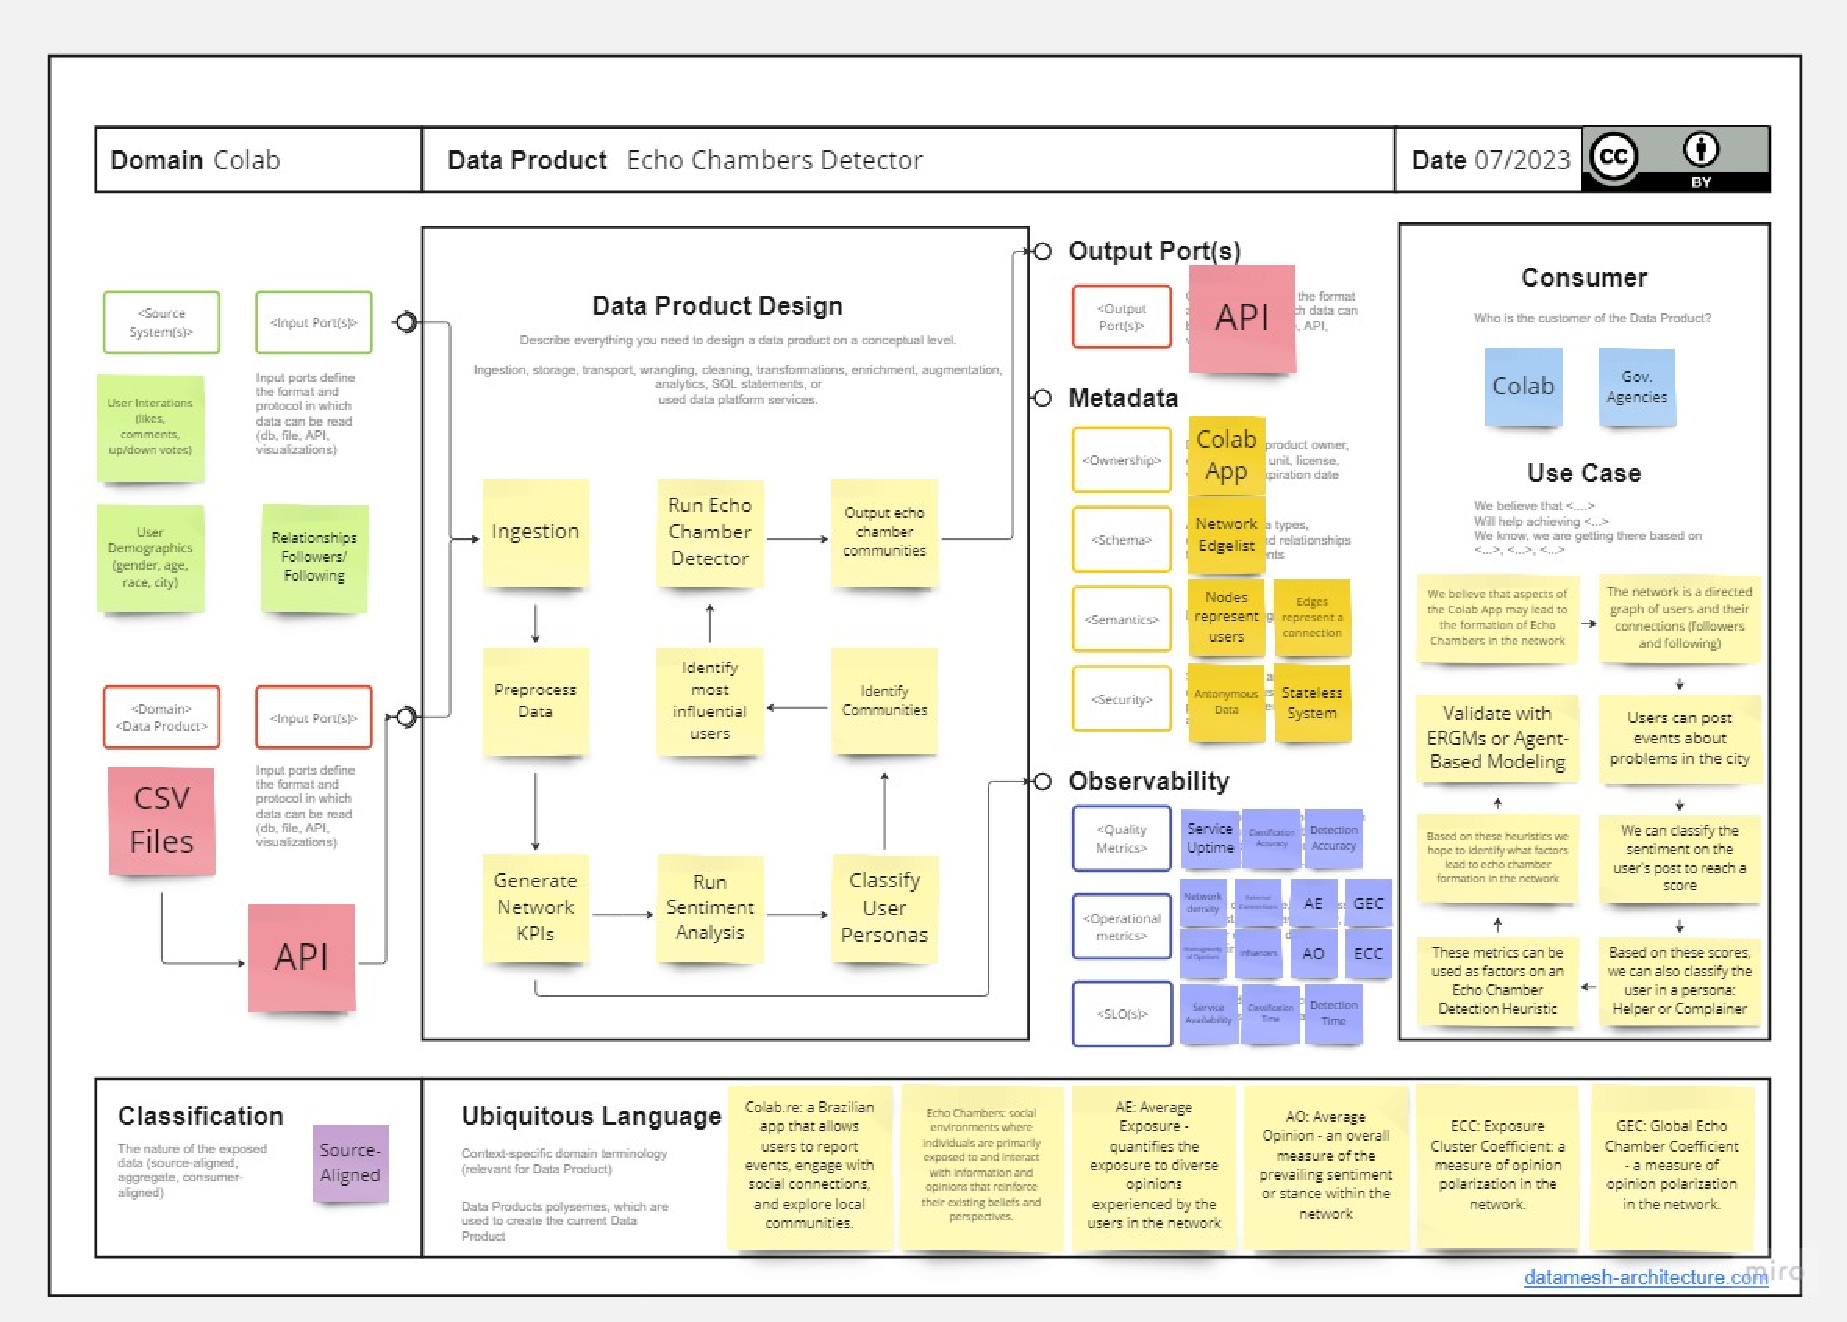
\includegraphics[width=0.9\textwidth]{tex/includes/data_canvas.pdf}
	\caption{Data Product Canvas desenvolvido para a estruturação do sistema de detecção de câmaras de eco.}
	\label{fig:data_canvas}
\end{figure}

Este instrumento emerge como um componente fundamental na aplicação das heurísticas de detecção de câmaras de eco em tempo real. O sistema concebido com base nesse canvas tem o potencial de fornecer alertas proativos aos administradores do Colab sobre emergentes câmaras de eco e tendências de polarização em tópicos específicos. A identificação precoce de tais fenômenos permite que os administradores adotem medidas preventivas e corretivas. Estratégias possíveis incluem a criação de novas categorias para postagens, a promoção de contribuições oriundas de perfis de usuários variados e a iniciação de tópicos de discussão inovadores, todos com o objetivo de mitigar a polarização e enaltecer a diversidade de opiniões dentro do ecossistema digital.

\subsection*{Validação de Conteúdo e a Gestão de Polarização nas Redes}

Ao discutir a implementação das heurísticas desenvolvidas em nesse estudo em sistemas de informação integrados ao Colab e num cenário onde sistemas automatizados ganham cada vez mais espaço na análise de interações em redes sociais, a reflexão sobre os mecanismos de moderação de conteúdo torna-se crucial. O desenvolvimento de métricas quantitativas e heurísticas para a identificação de indícios de polarização em redes digitais carrega consigo uma responsabilidade significativa. O objetivo primário de sistemas baseados nas heuristicas desse estudo deve ser a melhoria contínua dos serviços prestados pelo poder público nas cidades e o aprimoramento das plataformas de cidadania ativa, como o Colab.

As heurísticas de detecção de câmaras de eco e a análise de conteúdo postado pelos usuários, embora sofisticadas e valiosas, não podem operar isoladamente como juízes finais do que é considerado conteúdo polarizado. É imperativo que haja uma intervenção humana criteriosa, que atue como uma camada de validação final. Isto não apenas assegura a precisão e a relevância das conclusões do sistema, mas também protege contra a aplicação arbitrária de penalidades ou a remoção injustificada de conteúdo.

Por exemplo, a aplicação de punições ou a remoção de conteúdos baseada exclusivamente em critérios automatizados pode levar a erros de julgamento e a injustiças. Tais decisões, quando tomadas de forma precipitada e sem a devida análise humana, podem reprimir a liberdade de expressão e a diversidade de opiniões — valores essenciais em qualquer sociedade democrática. Portanto, é necessário estabelecer processos onde os resultados do sistema de detecção sejam sempre submetidos à avaliação de moderadores treinados, que possam interpretar as nuances e o contexto das interações, garantindo que as ações tomadas estejam em conformidade com as normas éticas e legais.

Além disso, a transparência nas práticas de moderação e a comunicação clara sobre como e por que certos conteúdos são sinalizados são fundamentais. Isso permite que os usuários compreendam as diretrizes da plataforma e participem ativamente na manutenção de um ambiente de debate saudável e construtivo. A implementação de sistemas de feedback onde os usuários podem contestar ações de moderação também contribui para a justiça e aperfeiçoamento contínuo dos algoritmos de moderação.

Ao contemplar a integração das heurísticas de detecção com outros sistemas, deve-se ponderar cuidadosamente sobre os limites e o alcance dessas integrações. A automação pode servir como uma ferramenta de triagem inicial, mas a decisão final deve sempre ser mediada pelo discernimento humano, com a finalidade de assegurar um equilíbrio entre a eficiência operacional e o respeito aos direitos dos indivíduos, afinal tecnologia deve estar a serviço da sociedade, e não o contrário. O desenvolvimento e implementação de qualquer sistema de análise de conteúdo em redes sociais, portanto, devem ser guiados por princípios éticos e pelo comprometimento com a promoção do bem comum, assegurando que as ferramentas digitais sejam utilizadas para enriquecer e não para limitar o discurso no cyberespaço.

\subsection*{Cyberespaço: Reflexo e Amplificador da Cultura Social}

A investigação dos padrões de interação no Colab e a detecção de câmaras de eco refletem um dos principais temas da "Cybercultura" de discutida em \citeonline{2010_Levy_BOOK}: a transformação das relações sociais mediadas pela tecnologia. Lévy argumenta que o cyberespaço é um novo meio de comunicação que altera significativamente a maneira como as informações são produzidas, transmitidas e consumidas.

Em linha com esta perspectiva, nossas descobertas sugerem que o Colab atua não apenas como uma plataforma para o engajamento cívico, mas também como um microcosmo do cyberespaço, onde fenômenos do mundo real encontram ecos nas interações digitais. A cada evento de zeladoria reportado com geolocalização no Colab, cria-se um simulacro digital, refletindo a concepção de \citeonline{1994_Baudrillard_BOOK} sobre a preponderância de representações sobre os objetos ou eventos que elas representam. Por exemplo, considere um bueiro entupido em Niterói. A prefeitura estabelece processos para agir em ocorrências dessa natureza a partir de reportes do Colab. Se um usuário reporta um bueiro entupido em Niterói através da plataforma, esse reporte não é apenas um registro de um problema urbano, mas também uma manifestação do problema no espaço digital. Portanto, para efeitos de correção do problema, esse bueiro não existe até que seja reportado e a cadeia de eventos delimitada pela prefeitura em resposta ao reporte possa ser iniciada. Nesse sentido, o Colab se torna um repositório de hiper-realidade, onde a experiência urbana é duplicada e, em alguns casos, a representação digital pode ganhar mais atenção e urgência do que a condição física que ela simboliza. Em outros casos, a falta de resposta por parte dos órgãos governamentais causam reportes de eventos muitas vezes duplicados uma ou mais vezes. Este espelho digital dos problemas urbanos não apenas reflete as questões do mundo real, mas também tem o potencial de moldar a percepção pública e a resposta política a essas questões.

Ao mapear as interações digitais no Colab, observamos como os usuários se tornam participantes ativos na construção dessa hiper-realidade, um processo que Levy poderia argumentar como sendo parte da sedução do ciberespaço, onde a simulação oferece uma nova forma de influência sobre a realidade. O Colab, portanto, não é apenas um reflexo da cidade, mas também um ator que pode transformar a maneira como problemas urbanos são percebidos e abordados. Por exemplo, usuários mais populares do colab podem trazer engajamento para questões que, de outra forma, não receberiam atenção. Além disso, a plataforma pode ser usada como uma ferramenta de \textit{advocacy}, onde os usuários podem se organizar para pressionar o governo a agir em relação a um problema específico.

Nesse sentido, os resultados da pesquisa apontam para o cyberespaço como um campo fértil para o florescimento de comunidades, mas também para a formação de câmaras de eco. As métricas e heurísticas desenvolvidas durante o estudo permitiram uma visão mais profunda sobre como as ideias e opiniões se propagam e como elas podem, em alguns casos, solidificar polarizações. Isso é particularmente relevante quando consideramos a noção de Lévy sobre a inteligência coletiva, que é potencializada no cyberespaço, mas que também depende da diversidade e da capacidade de diálogo entre seus participantes.

Ao mesmo tempo, a pesquisa destacou a necessidade de ferramentas que favoreçam a diversidade e o debate construtivo. Isso ressoa com o conceito de Lévy sobre a democracia eletrônica, na qual o cyberespaço pode ser um ambiente propício para a prática da democracia participativa, contanto que seja bem moderado e estruturado de maneira a promover a inclusão e o respeito mútuo.

Portanto, os insights obtidos do Colab ecoam com a visão de Lévy sobre a cybercultura, especialmente no que diz respeito ao papel da tecnologia na reconfiguração do espaço público e na promoção de uma cidadania ativa. A análise fenomenológica realizada nesta pesquisa, que observa o usuário como um agente de transformação, está alinhada com a ideia de que o cyberespaço é um ambiente participativo, onde cada indivíduo contribui para a forma e a substância da esfera pública digital.

Em conclusão, esse estudo não apenas explora a dinâmica das interações sociais no Colab, mas também se insere no contexto mais amplo da cybercultura, destacando como as tecnologias digitais podem ser utilizadas para refletir e, potencialmente, melhorar as práticas democráticas no cyberespaço. Assim como Lévy sugere, a chave para um futuro promissor reside na nossa capacidade de entender e aproveitar as oportunidades oferecidas por essas novas formas de comunicação para criar uma sociedade mais conectada, informada e engajada.

\section{Considerações Finais}

Neste estudo, empreendemos a tarefa de explorar o complexo ecossistema de interações dentro da rede social Colab, com o objetivo de compreender e prever comportamentos polarizadores e identificar câmaras de eco. As limitações inerentes ao nosso trabalho incluem a necessidade de refinar nosso modelo de classificação, a criação de pipelines para análise do conteúdo em tempo real e a incorporação de aspectos mais detalhados de geolocalização nas análises. Essas melhorias não apenas ampliarão a precisão de nossos resultados, mas também enriquecerão nossa compreensão da dinâmica das interações sociais digitais.

Um dos aspectos fascinantes revelados por nosso estudo é a emergência de subcomunidades, que por vezes se isolam do grafo principal, criando novos padrões de comunicação e interação. Investigar essas subcomunidades poderia lançar luz sobre como as ideias se propagam e como as bolhas de opinião são formadas e mantidas. Além disso, a extrapolação de nossas heurísticas para outras redes sociais poderia testar a robustez de nossas descobertas e talvez revelar universalidades nas dinâmicas de polarização e na formação de câmaras de eco.

Para estudos futuros, propomos a ampliação de nossa metodologia para captar dados em tempo real, o que permitiria uma análise ainda mais reativa e dinâmica. A integração de variáveis geoespaciais detalhadas poderia oferecer novas perspectivas sobre a influência do espaço físico nas interações virtuais, e vice-versa. A análise de redes sociais comparativas poderia proporcionar insights valiosos sobre as características únicas do Colab e sobre como diferentes plataformas podem moldar ou ser moldadas pela cidadania digital.

Este estudo entrelaçou disciplinas, desde a engenharia de software até a sociologia, e ressaltou a interseção entre a fenomenologia e a análise de dados. A polarização e as câmaras de eco não são fenômenos isolados no ciberespaço; são reflexos de uma sociedade que se debate com a disseminação de informações e a formação de opiniões. O Colab serviu como um observatório desses fenômenos, proporcionando uma plataforma para monitorar e, potencialmente, mitigar seus efeitos.

A fenomenologia nos ensinou a ver o usuário não apenas como um ponto de dados, mas como um agente de transformação cujas ações e interações moldam a realidade digital e física. A 'tecnificação das mãos', por sua vez, enfatiza a necessidade de ferramentas que nos permitam entender essa realidade complexa. O Colab, como uma microcosmo das realidades urbanas, ofereceu um campo vivo para a aplicação da engenharia de software e análise de redes no estudo da polarização e das câmaras de eco.

Em última análise, este trabalho não se limitou a traçar os contornos da polarização e das câmaras de eco, mas buscou compreender suas raízes e ramificações. Através da junção de ferramentas analíticas e percepção fenomenológica, esforçamo-nos para capturar a essência das interações humanas na era digital. A pesquisa revelou que, enquanto as tecnologias avançam e as redes se expandem, permanece a necessidade intrínseca de compreender como nos conectamos, comunicamos e nos polarizamos.

Portanto, gostariamos de deixar como legado não apenas um conjunto de heurísticas e acarbouços analíticos, mas uma filosofia de pesquisa que abraça a complexidade do ser humano no cerne da tecnologia. Que os futuros empreendimentos neste campo possam continuar a construir sobre esta base, ampliando nosso entendimento e melhorando a interação humana dentro e fora do ciberespaço. E que, em meio às ondas de dados e algoritmos, não esqueçamos que no centro de tudo estão as mãos humanas — tecendo, moldando e redefinindo o tecido de nossa coexistência digital e física.